\chapter[Diseño de la Plataforma]{Diseño de la Plataforma}
\label{Chap4}

La arquitectura planteada en la figura \ref{fig:ej9} es simple y fácil de implementar, pues scrapy mismo puede insertar los datos scrapeados de las web de forma directa en PostGreSQL, aunque presenta un problema. Djando hace uso de un sistema de gestión de versiones de los cambios realizados en la BBDD con el fin de reducir la carga de peticiones a la BBDD, esto se aplica desde el lado de Django, lo que supondría un problema a la hora de insertar datos directamente de Scrapy a PostGreSQL, pues los nuevos datos no serán detectados por Django, generando la situación de que una vez se vayan a pedir los nuevos datos, Django no devuelva nada, pues desde su punto de vista los datos anteriormente pedidos son la versión mas reciente, luego no es necesario realizar llamada alguna a la BBDD.

\begin{figure} [H]
	\centering
	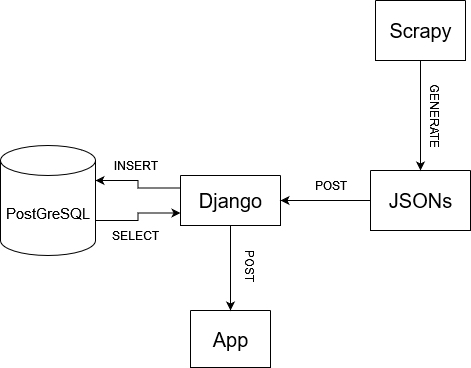
\includegraphics[width=0.4\textwidth]{fig/estructura_usada.png}
	\caption[Estructura de datos usada en el proyecto]{Estructura usada}
	\label{fig:ej10}
\end{figure}

Pasa solventar el problema, inicialmente se encontró el pluggin scrapy\_djangoitem, promete la comunicación entre scrapy y Django, pero se decidió no usarlo al llevar siete años sin revisiones. Como alternativa, se ha optado por la arquitectura de la figura \ref{fig:ej10}, que incluye un paso intermedio al almacenar los datos obtenidos de las distintas webs en formato JSON, para posteriormente enviárselos a Django, el cual se encargara de subir los datos a la BBDD.

\section{Trabajar con los Datos}

\begin{lstlisting}[caption={Flujo de datos}]
	Pedir datos
	Formatear datos
	Mandar datos a la BBDD
	Marcar datos como old
	
	While(true)
		Pedir datos
		Formatear datos
		Filtrar datos
		Mandar datos a la BBDD
		Marcar datos como old
\end{lstlisting}

El flujo que realizan los datos es el siguiente, inicialmente se pedirán los datos, como los datos obtenidos no son los mismos para cada web, se formatean para compartir una estructura heterogénea, en caso de ser la primera iteración, se mandan directamente los datos a la BBDD, de no ser la primera iteración, se filtran los nuevos datos de aquellos mascados como old (viejo), se envían los datos a la base de datos y, una vez enviados son marcados como old para ser el punto de comparación respecto a los datos que se obtendrán en la próxima iteración.

\subsection{Datos obtenidos por página}
Aemet:\newline
temperatura, humedad, precipitación
\newline\newline
meteoNavarra:\newline
temperatura, humedad, precipitación, radiación
\newline\newline
aguaEnNavarra:\newline
nivel, caudal
\newline\newline
chcantabrico:\newline
nivel, precipitación, seguimiento, alerta, pre-alerta
\newline\newline
En todas las webs se proporciona las coordenadas junto con la fecha y hora en la que se ha hecho la medida.

\subsection{Formato de Datos}
No todas las webs presentan sus datos de la misma manera, es por eso que nos encontramos con que los datos que hemos obtenido pueden llegar a estar repartidos en distintas páginas, haciendo necesario el uso de múltiples Spiders, resultando en multiples JSON.\newline
\newline
Debido a ello, para cada web se ha creado una función para parsear (formatear) los datos obtenidos, de esta manera se dispone de una estructura única para los datos recibidos, haciendo su uso posterior más fácil, ya sea a la hora de tratarlos como para almacenarlos en la base de datos.\newline
\newline
Esquema obtenido:

\begin{lstlisting}[language=json, basicstyle=\small]
[
{
	"coordenadas": "X. 598270,3 | Y. 4659333 | Z. 37928",
	"estacion": "64",
	"datos": [
	{
		"fecha y hora": "01/06/2023 11:20:00",
		"temperatura (C)": null,
		"humedad (%)": null,
		"precipitacion (mm)": null,
		"nivel (m)": "0,05",
		"caudal (m^3/s)": null,
		"radiacion (W/m^2)": null
	}
	]
}
]
\end{lstlisting}

\subsection{Filtrado de Datos}
Una vez formateados los datos, con el fin de reducir la carga a la base de datos, estos son filtrados mediante la comparación con los ficheros anteriormente marcados como old, de esta forma, nos aseguramos de mandar a la base de datos unicamente las instancias nuevas de los datos recogidos, pues no disponemos de ninguna manera de filtrar los datos a la hora de obtenerlos. Estos datos serán guardados en un tercer JSON.

\section{Arquitectura}
Para poder realizar el trabajo se ha diseñado la siguiente arquitectura.\ref{fig:ej7}

\begin{figure} [h]
	\centering
	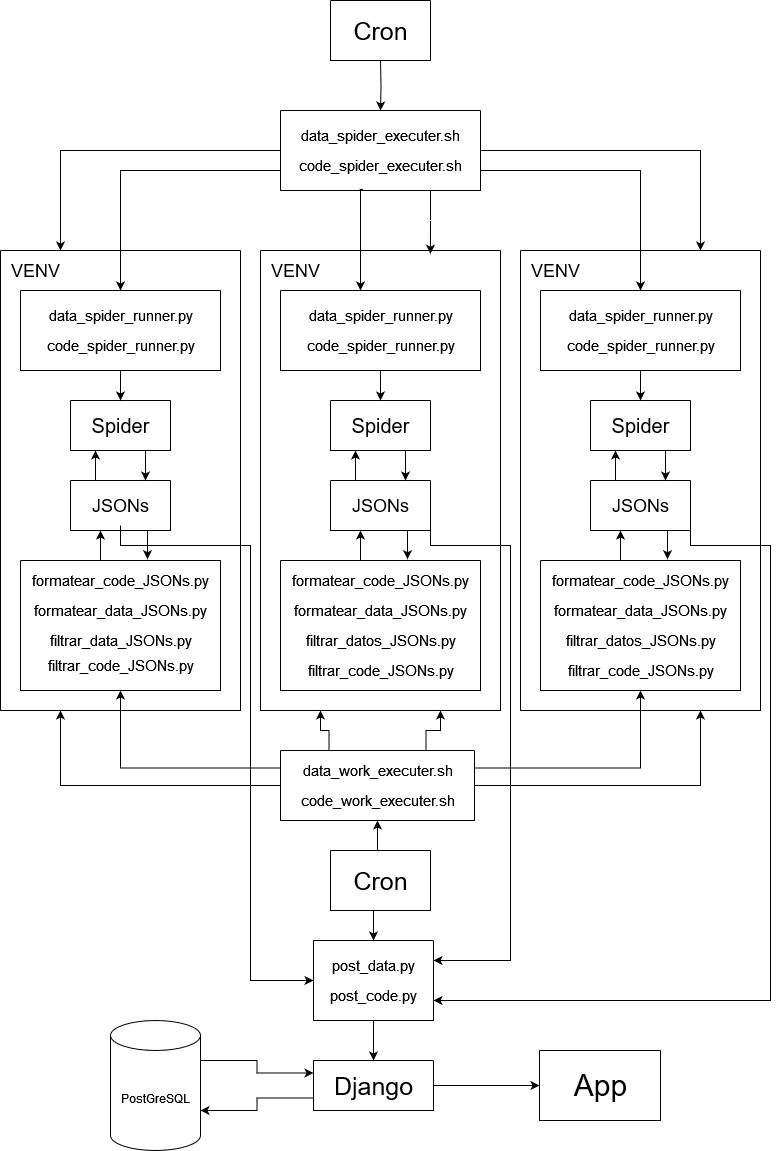
\includegraphics[width=0.7\textwidth]{fig/arquitectura.png}
	\caption[Arquitectura de obtención y tratamiento de datos]{Arquitectura de obtención y tratamiento de datos}
	\label{fig:ej7}
\end{figure}

\subsection{Entornos virtuales}
Con el fin de que la plataforma sea lo mas fácilmente ampliable, se ha decidido que cada Spider disponga de su propio entorno virtual, esto permite añadir dependencias de tal forma que no afecten a el resto de los scripts presentes, ayudando en la encapsulación de dependencias.\newline
\newline
Actualmente la plataforma dispone de cuatro entornos virtuales para cada Spider y un entorno virtual sobre el que ejecutar el servidor de Django.

\subsection{Spiders}
Cada Spider representa una web, de tal forma que cada una de ellas obtiene los datos de la web sobre la que se ha diseñado exclusivamente, para poder realizar esta tarea por cada web han sido necesarias varias Spider, aunque de forma simplificada se pueden agrupar por, aquellas que obtienen las estaciones junto con sus códigos y, las de obtención de datos.\newline
\newline
De esta forma, se dividen las tareas con la posibilidad de ejecutar aquella que mejor venga en cada momento.

\begin{figure} [H]
	\centering
	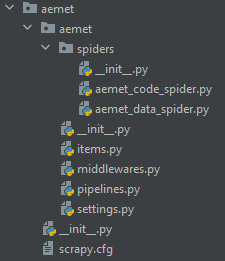
\includegraphics[width=0.3\textwidth]{fig/estructura_basica_spider.png}
	\caption[Estructuración básica de una Spider]{Estructuración básica de una Spider}
	\label{fig:ej8}
\end{figure}

\subsection{Runners}
Runner es la forma en la que han sido nombrados los Scripts cuya función es posibilitar la ejecución en nuestro caso asíncrona de una o múltiples Spiders mediante un único comando.\newline
\newline
Es un Script simple en el que una vez dispones de la estructura básica en caso de necesitar añadir o eliminar una Spider solo tienes que agregar o eliminar la Spider en cuestión y ya estaría listo.\newline
\newline
A su vez, al añadir un intermediario el comando de ejecución pasa de ser, scrapy crawl nombreSpider por cada Spider que se desea ejecutar, a, python nombreRunner.py facilitando la automatización de ejecución de las Spider.

\subsection{Executers}
Aumentado un poco mas la abstracción nos encontramos con los Executers, Scripts en Bash encargados de activar el entorno virtual de la Spider deseada y acto seguido ejecutar su respectivo Runner.\newline
\newline
Estos existen (en mayor medida que los Runners) con el fin de ayudar con el mantenimiento de la arquitectura, creando un nuevo intermediario en la cadena de ejecución.\newline
\newline
Están diseñados de tal forma que funcionen pasandoles un único argumento representando la web de la que quieres obtener los datos, haciendo que la agregación de nuevas Spiders junto con sus entornos sea tan sencillo como respetar las rutas y nombres predefinidos.

\subsection{Directorios de los JSONs de datos}
Este apartado es un conjunto de directorios en los que se van almacenando los JSON obtenidos tras los distintos procesos a los que son sometidos.\newline
\newline
Los directorios en cuestión, siguiendo orden de creación para los JSON de datos son los siguientes:

\begin{multicols}{2}
Directorios de los datos de estación:
\begin{enumerate}
	\item RawData
	\item ParsedData
	\item RefinedData
	\item OldData
\end{enumerate}

\columnbreak

Directorios de los códigos de estación:
\begin{enumerate}
	\item RawCode
	\item ParsedCode
	\item RefinedCode
	\item OldCode
\end{enumerate}
\end{multicols}

El primer nivel es aquel que almacena los JSON que genera la llamada con la Spider a la web. El segundo, los resultantes tras ejecutar ya sea formatear\_data\_JSONs.py en caso de querer parsear los datos o formatear\_code\_JSONs.py para los códigos. El tercero almacena los ficheros generados tras eliminar la duplicidad de datos en comparación con los ya almacenados en la base de datos, mediante la ejecución de filtrar\_data\_JSONs.py. Finalmente el cuarto guarda el fichero original ya formateado tras la comparación.

\subsection{Posts}
Estos Scripts son los encargado de enviar los datos mediante un Post Request al servidor Django.\newline
\newline
Diseñados bajo el mismo principio de fomentar la ampliabilidad del proyecto que los Executer, reciben el nombre de la web de la cual deseas enviar los datos a la hora de ejecutarlo junto al comando en forma de argumento.

\subsection{Cron}
Cron es un administrador regular de procesos en segundo plano presente en los sistemas basados en Unix. Con el es posible programar la automatización de ejecución de procesos en intervalos de tiempo, pudiendo indicar el minuto, hora, día, mes e incluso día de la semana.\newline
\newline
La especificación de los procesos se realiza en el archivo crontab y, su estructuración es la siguiente:

\begin{verbatim}
.--------------- minuto (0-59) 
|  .------------ hora (0-23)
|  |  .--------- día del mes (1-31)
|  |  |  .------ mes (1-12) o meses en inglés
|  |  |  |  .--- día de la semana (0-6) (domingo=0 o 7) o días en inglés 
|  |  |  |  |
*  *  *  *  *  comando a ejecutar
\end{verbatim}

En nuestro caso queremos el equivalente a dos instancias de Cron, una que se encargue de obtener los datos ya sea cada quince minutos, media hora y una hora manteniendo la base de datos actualizada para poder realizar las posteriores predicciones y otra que mensualmente compruebe la existencia de nuevas estaciones o el cese del uso de alguna de las ya disponibles.\newline
\newline
Así pues, Cron es el encargado de ejecutar cada proceso necesario dentro de la plataforma, ya sea, ejecutar las Spiders, los Scripts de formateo como de filtrado y, el envío de los datos a Django para su inserción en PostGreSQL.\newline
\newline
De esta forma dispondríamos de un sistema cerrado automático, el cual nos permitiría trabajar en otros apartados como puede ser la integración de mas webs en la plataforma o la mejora del sistema de predicción.

\subsection{API Django}
La instancia del servidor de Django es la encargada de tanto recibir los datos obtenidos como de enviarlos a la base de datos. Finalmente, una vez se dispusiera de una aplicación de predicción, se encargaría de pedir los datos almacenados y enviarlos mediante POST a la aplicación.

\subsection{Base de datos PostGreSQL}
La base de datos, dispone de las siguientes dos tablas de la figura \ref{fig:ej33}.

\begin{figure} [H]
	\centering
	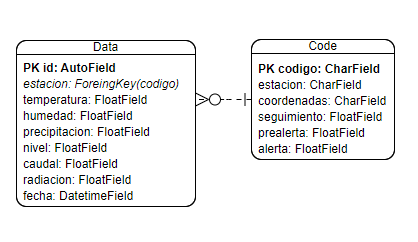
\includegraphics[width=0.7\textwidth]{fig/TablasBBDD.png}
	\caption[Tablas de la base de datos]{Tablas de la base de datos}
	\label{fig:ej33}
\end{figure}

Tienen una relación uno a muchos, siendo el campo estacion de la tabla Data la ForeingKey usada.\newline
\newline
Para la tabla Data, al almacenar miles de datos, se ha optado por usar una PrimaryKey auto incremental. A su vez, a excepción del campo fecha, cualquiera de los campos pueden ser nulos, pues cada web proporciona unicamente un conjunto de los datos.\newline
\newline
En la tabla Code, exceptuando la clave primaria y el nombre de la estación, el resto de campos tienen la posibilidad de ser nulos.

\section{Entorno de ejecución}
El proyecto se dividirá en dos ordenadores (maquinas virtuales). Uno de ellos será el responsable de la base de datos en PostGreSQL, mientras que, el otro, se encargara de la ejecución del código de obtención de datos, tratarlos y enviarlos a la base de datos.

\subsection{Preparación de entorno virtual}
Primero instalaremos las dependencias para crear y activar un entorno virtual sobre el que trabajar, para ello ejecutaremos los siguientes comandos:

\begin{lstlisting}
	#Instalamos las dependencias
	user@host:~$ sudo apt install python3-venv python3-dev
	
	#Creamos un nuevo directorio sobre el que trabajar
	user@host:~$ mkdir ~/dirdemiproyecto
	user@host:~$ cd ~/dirdemiproyecto
	
	#Creamos el entorno virtual
	user@host:~/dirdemiproyecto$ python3 -m venv envdemiproyecto
	
	#Activamos el entorno virtual
	user@host:~/dirdemiproyecto$ source envdemiproyecto/bin/activate
	
	#Una vez seguidos los pasos nuestra terminal debe mostrarse asi
	(envdemiproyecto) user@host:~/dirdemiproyecto$
\end{lstlisting}

Cada Spider dispondrá de su propio entorno virtual, nombrado tras la pagina web a la que representa, de esta forma, por ejemplo, el entorno virtual para la web de CHcantábrico se llamará chcantabrico. Otro entorno virtual es usado para el servidor Django y los scripts encargados del envío de datos.

\subsection{Instalación y configuración de PostGreSQL}
Los comandos necesarios para la instalación inicial de PostGreSQL, la creación de un usuario y una base de datos son.

\begin{lstlisting}
	#Instalamos PostGreSQL y las dependencias
	user@host:~$ sudo apt install libpq-dev postgresql postgresql-contrib
	
	#Iniciamos sesion usando el role postgres y accedemos a PostGreSQL
	user@host:~$ sudo -u postgres psql
	
	#Si todo esta bien la terminal deberia mostrarse asi
	postgres=# 
	
	#Creamos un nuevo usuario
	postgres=# CREATE USER miusuario WITH PASSWORD 'micontrasena';
	
	#Configuramos varios parametros del usuario para una mejor integracion con Django
	postgres=# ALTER ROLE miusuario SET client_encoding TO 'utf8';
	postgres=# ALTER ROLE miusuario SET default_transaction_isolation TO 'read committed';
	postgres=# ALTER ROLE miusuario SET timezone TO 'Europe/Madrid';
	
	#Creamos la Base de Datos
	postgres=# CREATE DATABASE bbddmiproyecto;
	
	#Otorgamos permisos de administrador a nuestro usuario en la base de datos
	postgres=# GRANT ALL PRIVILEGES ON DATABASE bbddmiproyecto TO miusuario;
	
	#Una vez finalizado
	postqres=# \q
\end{lstlisting}

En este punto ya se dispondría de una base de datos (aun sin tablas en ella) y de un usuario con el que conectarse a esta desde Django.\newline
\newline
Ahora quedaría configurar el permiso de comunicación entre dispositivos, más concretamente la conexión remota de Django con PostGreSQL.

\begin{lstlisting}
	#Abrimos el archivo postgresql.conf con un editor
	user@host:~$ sudo nano /etc/postgresql/11/main/postgresql.conf
	
	#Buscamos la linea "#listen_addresses = 'localhost'", borramos la almohadilla y
	sustituimos localhost por *, permitiendo la escucha de cualquier direccion IP
	listen_addresses = '*'
	
	#Guardamos y cerramos el fichero
	
	#Abrimos el archivo pg_hba.conf con un editor
	user@host:~$ sudo nano /etc/postgresql/11/main/pg_hba.conf
	
	#Por defecto solo permite conexiones desde localhost
	# IPv4 local connections: 
	host    all             all             127.0.0.1/32            md5 
	
	#Configuararemos el permiso de conexion remota desde cualquier IP añadiendo
	la siguiente linea debajo de la anterior
	host    all             all             0.0.0.0/0            md5 
	
	#O podemos configurar el permiso unicamente para la IP de la otra maquina virtual
	host    all             all             127.18.83.198/19            md5 
	
	#Guardamos y cerramos el fichero
	
	#Finalmete permitimos el trafico mediante el puerto 5432 (puesto por defecto)
	user@host:~$ sudo ufw allow 5432/tcp
\end{lstlisting}

Una vez realizados los siguientes pasos ya está la instancia de PostGreSQL configurada.

\subsection{Instalación y configuración de Django}
Antes de instalar Django, es necesario generar un entorno virtual sobre el que trabajar.

\begin{lstlisting}
	#Instalamos Django y las dependencias
	(envdemiproyecto) user@host:~/dirdemiproyecto$ pip install django psycopg2
	
	#Creamos un nuevo proyecto de Django
	(envdemiproyecto) user@host:~/dirdemiproyecto$ django-admin startproject djangoAPI
	(envdemiproyecto) user@host:~/dirdemiproyecto$ cd djangoAPI
	
	#Creamos una nueva app Django
	(envdemiproyecto) user@host:~/dirdemiproyecto/djangoAPI$ python manage.py startapp appAPI
\end{lstlisting}

Una vez realizado lo siguiente, quedaría configurar la API.

\begin{lstlisting}
	#Abrimos el archivo settings.py con un editor
	(envdemiproyecto) user@host:~/dirdemiproyecto/djangoAPI$ nano djangoAPI/settings.py
	
	#Añadimos nuestra app en la lista de INSTALLED_APPS
	INSTALLED_APPS = [
		'django.contrib.admin',
		'django.contrib.auth',
		'django.contrib.contenttypes',
		'django.contrib.sessions',
		'django.contrib.messages',
		'django.contrib.staticfiles',
		'appAPI.apps.AppapiConfig',
	]
	
	#Configuramos la base de datos sutituyendo
	DATABASES = {
		'default': {
			'ENGINE': 'django.db.backends.sqlite3',
			'NAME': os.path.join(BASE_DIR, 'db.sqlite3'),
		}
	}

	por

	DATABASES = {
		'default': {
			'ENGINE': 'django.db.backends.postgresql_psycopg2',
			'NAME': 'bbddmiproyecto',
			'USER': 'miusuario',
			'PASSWORD': 'micontrasena',
			'HOST': '172.18.83.197',
			'PORT': '5432',
		}
	}

	#Configuramos las IP admitidas
	ALLOWED_HOSTS = ['172.18.83.197', 'localhost']
	
	#Configuramos la zona horaria
	TIME_ZONE = 'Europe/Madrid'
	
	#Configuramos el tamaño maximo de datos a None, con el fin de poder
	enviar cualquier cantidad de datos
	DATA_UPLOAD_MAX_MEMORY_SIZE = None
	
	#Guardamos y cerramos el fichero
	
	#Finalmete permitimos el trafico mediante el puerto 8000 (puesto por defecto)
	user@host:~$ sudo ufw allow 8000
\end{lstlisting}

Tras configurar la API, toca crear los modelos de la base de datos.

\begin{lstlisting}
	#Abrimos el archivo models.py dentro de la carpeta appAPI con un editor
	(envdemiproyecto) user@host:~/dirdemiproyecto/djangoAPI$ nano appAPI/models.py
\end{lstlisting}

Dentro definimos los modelos Data y Code.

\begin{lstlisting}[language=Python, caption={Modelos API Django}]
	from django.db import models
	
	class Data(models.Model):
		temperatura = models.FloatField(null=True)
		humedad = models.FloatField(null=True)
		precipitacion = models.FloatField(null=True)
		nivel = models.FloatField(null=True)
		caudal = models.FloatField(null=True)
		radiacion = models.FloatField(null=True)
		fecha = models.DateTimeField()
		estacion = models.ForeignKey("Code", on_delete=models.CASCADE)
	
	class Code(models.Model):
		estacion = models.CharField(max_length=50)
		codigo = models.CharField(max_length=20, primary_key=True)
		coodenadas = models.CharField(max_length=50)
		seguimiento = models.FloatField(null=True)
		prealerta = models.FloatField(null=True)
		alerta = models.FloatField(null=True)
\end{lstlisting}

Para importar los modelos a la base de datos, con el fin de crear las respectivas tablas.

\begin{lstlisting}
	#Actualizamos los datos realizados en models.py
	(envdemiproyecto) user@host:~/dirdemiproyecto$ python3 manage.py makemigrations
	
	#Migramos los datos
	envdemiproyecto) user@host:~/dirdemiproyecto$ python3 manage.py migrate
\end{lstlisting}

Si se quiere confirmar la correcta creación de las tablas, desde la terminal de PostGre.

\begin{lstlisting}
	#Nos conectamos a la base de datos
	postgres=# \c bbddmiproyecto
	
	#Mostramos las tablas
	postgres=# \d
\end{lstlisting}

Si todo a ido bien, se deberían mostrar como en la figura \ref{fig:ej34}.

\begin{figure} [H]
	\centering
	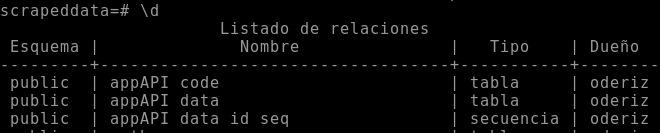
\includegraphics[width=0.6\textwidth]{fig/comprobacionTablasBBDD.png}
	\caption[Lista de tablas en PostGreSQL]{Lista de tablas en PostGreSQL}
	\label{fig:ej34}
\end{figure}

Tras configurar la API y crear las tablas de la base de datos, se creará la API como tal.

\begin{lstlisting}
	#Creamos el archivo urls.py con un editor dentro de la carpeta appAPI
	(envdemiproyecto) user@host:~/dirdemiproyecto/djangoAPI$ nano appAPI/urls.py
\end{lstlisting}

Dentro se incluye el siguiente código.

\begin{lstlisting}[language=Python, caption={Definición URLs API}]
	from django.urls import path
	from django.views.decorators.csrf import csrf_exempt
	
	from . import views

	urlpatterns = [
		path("storeData", csrf_exempt(views.storeData), name="storeData"),
		path("storeCode", csrf_exempt(views.storeCode), name="storeCode"),
	]
\end{lstlisting}

Aquí se definen las rutas para realizar una llamada a la API, en este caso storeData y storeCode.\newline
\newline
Si se quiere que el proyecto tenga constancia de ellas.

\begin{lstlisting}
	#Abrimos el archivo urls.py dentro de la carpeta djangoAPI con un editor
	(envdemiproyecto) user@host:~/dirdemiproyecto/djangoAPI$ nano djangoAPI/urls.py
\end{lstlisting}

Dentro se incluye el siguiente código.

\begin{lstlisting}[language=Python, caption={Configuración URLs API}]
	from django.contrib import admin
	from django.urls import path, include
	
	urlpatterns = [
		path('admin/', admin.site.urls),
		path('appapi/', include('appapi.urls'))
	]
\end{lstlisting}

Para finalizar, se crean las vistas a las que dirigen las rutas.

\begin{lstlisting}
	#Abrimos el archivo views.py dentro de la carpeta appAPI con un editor
	(envdemiproyecto) user@host:~/dirdemiproyecto/djangoAPI$ nano appAPI/views.py
\end{lstlisting}

Dentro se incluye el siguiente código.

\begin{lstlisting}[language=Python, caption={Definición funciones de recepción y almacenamiento de datos API}]
	import json
	
	from django.http import JsonResponse
	from .models import Data, Code
	
	# Create your views here.
	def storeData(request):
		data = json.loads(request.body.decode("utf-8"))
		for estacion in data:
			for datos in estacion['datos']:
				dato = Data(
					temperatura=datos['temperatura (ºC)'],
					humedad=datos['humedad (%)'],
					precipitacion=datos['precipitacion (mm)'],
					nivel=datos['nivel (m)'],
					caudal=datos['caudal (m^3/s)'],
					radiacion=datos['radiacion (W/m^2)'],
					fecha=datos['fecha y hora'],
					estacion=estacion['estacion']
				)
			dato.save()
		return JsonResponse(data, safe=False)
	
	def storeCode(request):
		data = json.loads(request.body.decode("utf-8"))
		for estacion in data:
			dato = Code(
				estacion=estacion['estacion'],
				codigo=estacion['codigo'],
				coodenadas=estacion['coodenadas'],
				seguimiento=estacion['seguimiento'],
				prealerta=estacion['prealerta'],
				alerta=estacion['alerta'],
			)
		dato.save()
	return JsonResponse(data, safe=False)
\end{lstlisting}

Estas funciones se encargan de recibir los datos enviados, iterar por ellos y subirlos a la base de datos con el método \textit{save()}.\newline
\newline
Con esto concluiría la creación y configuración de la API.
